\documentclass{beamer}
\usetheme{Madrid}
\usepackage{lmodern}% http://ctan.org/pkg/lm
\setbeamersize{text margin left = 2.5em}
\setbeamersize{text margin right = 2.5em}
\usepackage{color}
\usepackage{graphicx}
\usepackage{MnSymbol}
\usepackage{amsmath}
\usepackage{comment}
\usepackage{tikz}
\usepackage{subfigure}
\usepackage{listings}
\usetikzlibrary{automata}

%\usepackage[backend=bibtex,sorting=none]{biblatex}
%\addbibresource{E:/Papers/LiuLab} %BibTeX�����ļ���λ��
%\setbeamerfont{footnote}{size=\tiny}
\setbeamertemplate{theorems}[numbered]
\setbeamertemplate{caption}[numbered]
%% ʹ�ý�ע���õ�Ƭijҳ���Ӳο����ס�
%% ��������ʹ�ã�\footfullcite{bib_item} %����item
%% \usepackage{anyfontsize}%% allowing font sizes at arbitrary sizes
\logo{
\includegraphics[height=0.05\textwidth]{Pic/logo}}
\newtheorem{df}{Definition}
\newtheorem{DF}{DEFINITION}
\newtheorem{prop}{Proposition}
\newtheorem{thm}{Theorem}
\newtheorem{cor}{COROLLARY}
\newtheorem{lm}{LEMMA}
% ----------------------------------------------------------------------------------------
% TITLE PAGE
% ----------------------------------------------------------------------------------------

\title{P03 Planning and Uncertainty}
% The short title appears at the bottom of every slide, the full title is only on the title page

\author{Suixin Ou} % Your name
\institute[SYSU] % Your institution as it will appear on the bottom of every slide, may be shorthand to save space
{
  School of Computer Science\\
  Sun Yat-sen University \\ % Your institution for the title page
  \medskip
  % Your email address
}

\date{November 30, 2021} % Date, can be changed to a custom date

\AtBeginSection[]
{
  \begin{frame}
    \tableofcontents[currentsection,currentsubsection]
  \end{frame}
}

\begin{document}

\begin{frame}
  \titlepage
\end{frame}

\begin{frame}
  \frametitle{STRIPS Planner}
  \begin{block}{Problem 1}
In this part, you will implement a simple STRIPS planner.
\begin{itemize}
    \item  Input: the input of your planner is a PDDL domain file and a problem file in the STRIPS restriction, that is, preconditions of actions and the goal are conjunctions of atoms, and effects of actions are conjunctions of literals. 

    \item Output: the output of your planner is a sequence of actions to achieve the goal.
    \end{itemize}
  \end{block}
\end{frame}


\begin{frame}
  \frametitle{STRIPS Planner}

  \begin{block}{Grading}
    \begin{itemize}

\item Describe with sentences the main ideas behind computing the heuristic for a state using reachability analysis from lecture notes. (20 points)
    

\item Implement a STRIPS planner by using A$^*$ search and the heuristic function you implemented.(40 points)

\item Explain any ideas you use to speed up the implementation. (20 points)

\item Run you planner on the 5 test cases, and report the returned plans and the running times. Analyse the experimental results. (20 points)
    \end{itemize}
  \end{block}
\end{frame}


\begin{frame}
  \frametitle{Diagnosing by Bayesian Networks}
  \begin{block}{Problem 2}

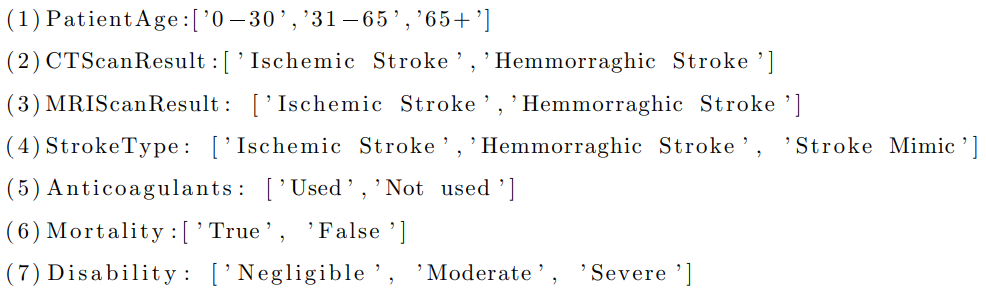
\includegraphics[width=10cm]{Pic/e21}
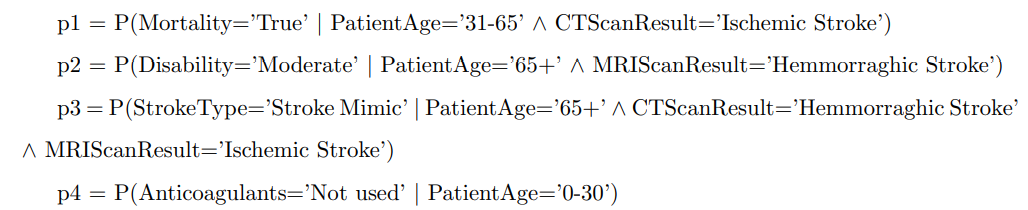
\includegraphics[width=10cm]{Pic/e22}
  \end{block}
\end{frame}



\begin{frame}
  \frametitle{Diagnosing by Bayesian Networks}

  \begin{block}{Grading}
\begin{itemize}
\item Briefly describe with sentences the main ideas of  the VE algorithm. (20 points)

\item Implement the VE algorithm (C++ or Python) to calculate the following probability values: (20 points)
    
\begin{enumerate}
\item p1 = P(Mortality='True' $\land$ CTScanResult='Ischemic Stroke' $|$ PatientAge='31-65' )

\item p2 = P(Disability='Moderate' $\land$ CTScanResult='Hemmorraghic Stroke' $|$ PatientAge='65+' $\land$  MRIScanResult='Hemmorraghic Stroke')

\item p3 = P(StrokeType='Hemmorraghic Stroke' $|$ PatientAge='65+' $\land$ CTScanResult='Hemmorraghic Stroke' $\land$ MRIScanResult='Ischemic Stroke')

\item p4 = P(Anticoagulants='Used' $|$ PatientAge='31-65')

\item p5 = P(Disability='Negligible')
\end{enumerate}



    \end{itemize}
  \end{block}
\end{frame}





\begin{frame}    

  \frametitle{Diagnosing by Bayesian Networks}

  \begin{block}{Grading}
\begin{itemize}


\item Implement an algorithm to select a good order of variable elimination. (20 points)
\item Compare the running times of the VE algorithm for different orders of variable elimination, and fill out the following table: For test cases p4 and p5, for each of the order selected by your algorithm and 5 other orders, report the elimination with, and the total running time of the VE algorithm. For each case, the first order of elimination should be the one chosen by your algorithm. Analyze the results. (40 points)
    

\end{itemize}
  \end{block}


\end{frame}





\begin{frame}    

  \frametitle{Diagnosing by Bayesian Networks}

  \begin{block}{Grading}

    \begin{tabular}{|c|c|c|c|}
\hline
Test case                                                                                             & Elimination order & Elimination width  & Total time \\ \hline
p4  & &  &            \\ \hline
p4  & &  &            \\ \hline
p4  & &  &            \\ \hline
p4  & &  &            \\ \hline
p4  & &  &            \\ \hline
p4  & &  &            \\ \hline
p5  & &  &            \\ \hline
p5  & &  &            \\ \hline
p5  & &  &            \\ \hline
p5  & &  &            \\ \hline
p5  & &  &            \\ \hline
p5  & &  &            \\ \hline
\end{tabular} 
  \end{block}


\end{frame}


\begin{frame} \frametitle{Task}
  \begin{block}{Submission}
    \begin{itemize}
      \item \textbf{Just choose one problem to solve.} There is no bonus even if you complete both the two tasks. You should finish one of them as well as you can.
\item Pack your report \texttt{P03\_YourNumber.pdf} and source code into zip file \texttt{P03\_YourNumber.zip}, then send it to \texttt{ai\_course2021@163.com}.

    \end{itemize}

    
  \end{block}
\end{frame}



%-----------------------------------------------------------------------------------------

\begin{frame}
  \Huge{\centerline{The End}}
\end{frame}

% ----------------------------------------------------------------------------------------


\end{document}
